\documentclass{article}
\usepackage{graphicx} % Required for inserting images
\usepackage{geometry}
\usepackage[utf8]{inputenc}
\usepackage{fancyhdr}  % Added package for headers and footers
\usepackage{amsmath}
\usepackage{subcaption}

% HEADER & FOOTER
\pagestyle{fancy}
\fancyhf{}
\setlength\headheight{15pt}

% Set the header offset to manually adjust the header width
\fancyheadoffset[L]{0.4cm}

\fancyhead[L]{Control and Computer Applications - EEP311}
\fancyhead[R]{Report DACs}
\fancyfootoffset[L]{0.4cm}
\renewcommand{\footrulewidth}{0.4pt}  % Add this line for a line above the footer
\fancyfoot[L]{20010099 - Ahmed Samy}
\fancyfoot[C]{\thepage}

\geometry{left=2cm , right=2cm , top=2 cm , bottom=2cm}
\newcommand{\HRule}[1]{\rule{\linewidth}{#1}}



%%%%%%%%%%%%%%%%%%%%%%%%%%%%%%%%%%%%%%%%%%
\title{ \normalsize \textsc{Control and Computer Applications - EEP311}
		\\ [2.0cm]
		\HRule{4pt} 
		\LARGE \textbf{\uppercase{Comprehensive Review on Digital to Analog Converters: From Fundamental Principles to Advanced ICs}}
		\HRule{2pt} \\[0.5cm]
		\normalsize \today \vspace*{5\baselineskip}}
\date{}

%%%%%%%%%%%%%%%%%%%%%%%%%%%%%%%%%%%%%%%%%%

\author{
\fontsize{14}{16}\selectfont\textbf{Name: Ahmed Samy Mohammed Elnozahy}\\
\\
		\fontsize{14}{16}\selectfont\textbf{ID: 20010099} \\
  }

%%%%%%%%%%%%%%%%%%%%%%%%%%%%%%%%%%%%%%%%%%

\begin{document}

\begin{figure}
    \centering
    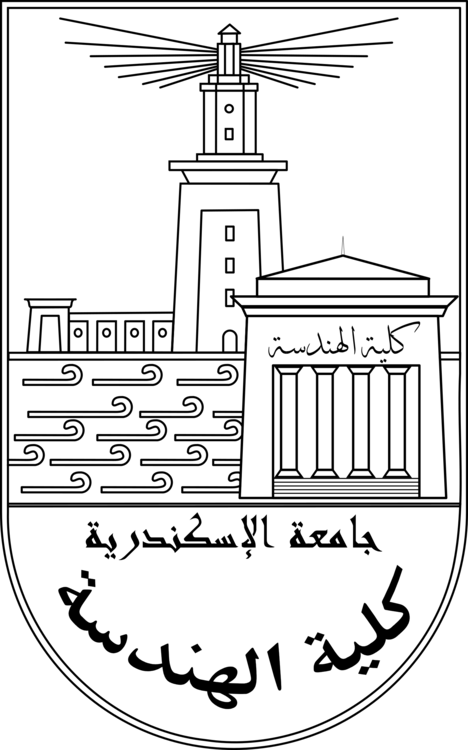
\includegraphics[width=0.1\linewidth]{logo.png}
\end{figure}
\maketitle

%%%%%%%%%%%%%%%%%%%%%%%%%%%%%%%%%%%%%%%%%%


\newpage
\tableofcontents
\newpage
%%%%%%%%%%%%%%%%%%%%%%%%%%%%%%%%%%%%%%%%%%
\section{Introduction}
\fontsize{14}{16}\selectfont
The report explores Digital to Analog Converters (DACs) with a specific emphasis on two types: Binary-Weighted Resistor (BWR) and R-2R ladder architectures. The DAC 7821 IC, featuring the R-2R ladder, is a central focus. This investigation aims to elucidate the principles, distinctions, and applications of these DAC types in contemporary electronic circuits.
%%%%%%%%%%%%%%%%%%%%%%%%%%%%%%%%%%%%%%%%%%
\section{Binary-Weighted Resistor (BWR)}
\fontsize{14}{16}\selectfont
\subsection{Basic Principle:}

Utilizes weighted resistors and an inverting amplifier op-amp.
Each resistor represents a digital bit, converting it into an analog form.
Works from the Least Significant Bit (LSB) to the Most Significant Bit (MSB).
%%%%%%%%%%%%%%%%%%%%%%%%%%%%%%%%%%%%%%%%%%
\subsection{DAC Working:}

Takes digital input, transforms it into proportional analog output.
Output voltage depends on the binary code input.
Involves a summing operational amplifier and weighted resistors.
%%%%%%%%%%%%%%%%%%%%%%%%%%%%%%%%%%%%%%%%%%
\subsection{Resolution and Step Size:}

\subsubsection{Resolution:}
Resolution is a fundamental parameter that defines the ability of a DAC to represent a range of analog value

\begin{equation}
Resolution = 2^n
\end{equation}
%%%%%%%%%%%%%%%%%%%%%%%%%%%%%%%%%%%%%%%%%%
\subsubsection{Step Size:}

Step size is the smallest change in output voltage that a DAC can produce.
It represents the difference between two consecutive voltage levels of the DAC.
The relationship between resolution (R) and step size 
is given by: 

\begin{equation}
Step Size = \frac{V_{ref}}{2^n}
\end{equation}
\newpage

%%%%%%%%%%%%%%%%%%%%%%%%%%%%%%%%%%%%%%%%%%
\subsection{\textbf{Summing amplifier configuration.}}
A summing amplifier adds weighted input voltages to produce an output voltage.
Binary input is applied through digital switches, each corresponding to a bit in the binary code.
These switches alter the reference voltage seen by the summing amplifier, influencing the output.
%%%%%%%%%%%%%%%%%%%%%%%%%%%%%%%%%%%%%%%%%%
\subsubsection{BWR Circuit}

\begin{figure}[htbp]
    \centering
    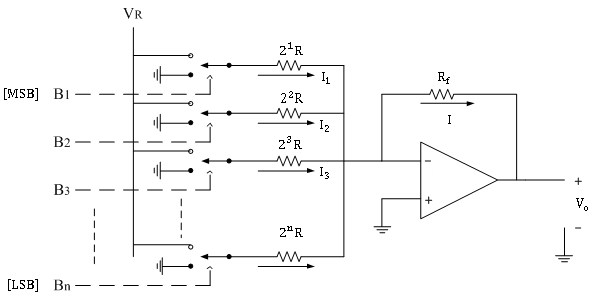
\includegraphics[width=0.5\linewidth]{bw.png}
    \caption{Binary-Weighted Resistor Circuit}
    \label{fig:enter-label}
\end{figure}
%%%%%%%%%%%%%%%%%%%%%%%%%%%%%%%%%%%%%%%%%%
\subsubsection{Output Voltage Formula}


\begin{equation}
\fontsize{10}{6}\selectfont
V_{out} = R_f\cdot I_0
\end{equation}
as: 
\begin{equation}
\fontsize{10}{6}\selectfont
I_0 = V_{ref} \sum_{i=1}^N \frac{b_i}{2^{i-1} R}
\end{equation}
also: 
\begin{equation}
\fontsize{10}{6}\selectfont
V_{out} = - V_{ref}(B_0 \frac{R_f}{R_0} + B_1 \frac{R_f}{R_1} ... + B_{n-1} \frac{R_f}{R_n-1})
\end{equation}

%%%%%%%%%%%%%%%%%%%%%%%%%%%%%%%%%%%%%%%%%%
\subsubsection{Example:}
For a specific scenario with a 4-bit DAC and given parameters:

\begin{itemize}
    \item \( V_{\text{ref}} = 5 \, \text{V} \) , Binary code: \( 1011 \)
\end{itemize}

The calculated output voltage (\( V_{\text{out}} \)) is given by the formula:


{\fontsize{10}{6}\selectfont
\begin{equation}
    V_{\text{out}} = -5 \left( 1 \cdot \frac{1}{2^3} + 0 \cdot \frac{1}{2^2} + 1 \cdot \frac{1}{2^1} + 1 \cdot \frac{1}{2^0} \right)
\end{equation}

\begin{equation}
    V_{\text{out}} = -5 \left( \frac{1}{8} + 0 + \frac{1}{2} + 1 \right)
\end{equation}

\begin{equation}
    V_{\text{out}} = -6.875 \, \text{V}
\end{equation}
}
%%%%%%%%%%%%%%%%%%%%%%%%%%%%%%%%%%%%%%%%%%
\subsection{Drawbacks and Advantages}

\subsubsection{Drawbacks}
\begin{itemize}
    \item Precision challenges for higher-order DAC, Temperature-dependent stability.
\end{itemize}

\subsubsection{Advantages}
\begin{itemize}
    \item Simple assembly, Fast conversion speed, Straightforward circuitry.
\end{itemize}


\section{The R-2R ladder network}
\fontsize{14}{16}\selectfont
%%%%%%%%%%%%%%%%%%%%%%%%%%%%%%%%%%%%%%%%%%
\subsection{ 4-bit R-2R Circuit}

\begin{figure}[h]
    \centering
    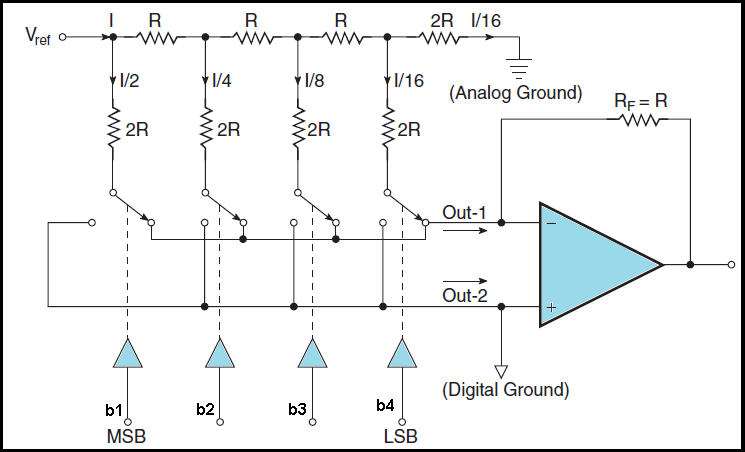
\includegraphics[width=0.4\linewidth]{r2r.png}
    \caption{4-bit R-2R Resistive Ladder Network}
    \label{fig:r2r}
\end{figure}
\subsection{Working Principle}

The R-2R ladder network operates on the principle of superposition and linearity. Each bit of the digital input contributes to a fraction of the total output voltage. The binary-weighted structure simplifies the design and ensures accurate conversion.

%%%%%%%%%%%%%%%%%%%%%%%%%%%%%%%%%%%%%%%%%%
\subsection{Output Voltage Formula}

The output voltage (\(V_{\text{out}}\)) in an R-2R ladder DAC is given by the equation:

\[\fontsize{10}{6}\selectfont
V_{\text{out}} = -V_{\text{ref}} \left(1 - \frac{1}{2^n}\right)
\]

This formula illustrates the relationship between the output voltage, reference voltage (\(V_{\text{ref}}\)), and the number of bits (\(n\)) in the DAC. As the number of bits increases, the output voltage approaches \(-V_{\text{ref}}\), providing a valuable insight into the DAC's resolution.
%%%%%%%%%%%%%%%%%%%%%%%%%%%%%%%%%%%%%%%%%%
\subsection{4-bit R-2R Ladder Example}

Consider a 4-bit R-2R ladder network with a reference voltage \(V_{\text{ref}} = 5 \, \text{V}\). The output voltage (\(V_{\text{out}}\)) is given by the formula:

\[\fontsize{10}{6}\selectfont
V_{\text{out}} = -5 \left( \frac{B_0}{2^0} + \frac{B_1}{2^1} + \frac{B_2}{2^2} + \frac{B_3}{2^3} \right)
\]

For a binary input of \(1011\), the calculated output voltage is:

\[\fontsize{10}{6}\selectfont
V_{\text{out}} = -5 \left( \frac{1}{1} + \frac{1}{2} + \frac{0}{4} + \frac{1}{8} \right)
\]

\[\fontsize{10}{6}\selectfont
V_{\text{out}} = -5 \left( 1 + 0.5 + 0 + 0.125 \right)
\]

\[\fontsize{10}{6}\selectfont
V_{\text{out}} = -6.625 \, \text{V}
\]
%%%%%%%%%%%%%%%%%%%%%%%%%%%%%%%%%%%%%%%%%%
\subsection{Advantages}

\begin{itemize}
    \item Reduced component count compared to other DAC architectures, Easy scalability for different resolutions.
\end{itemize}

\subsection{Disadvantages}

\begin{itemize}
    \item Limited to low to medium resolutions, Requires precision resistors for accurate conversion.
\end{itemize}
%%%%%%%%%%%%%%%%%%%%%%%%%%%%%%%%%%%%%%%%%%
\newpage
%%%%%%%%%%%%%%%%%%%%%%%%%%%%%%%%%%%%%%%%%%

\section{DAC7821 Integrated Circuit (IC)}
\fontsize{14}{16}\selectfont

\subsection{Overview}

The DAC7821 is a 12-bit Digital to Analog Converter (DAC) IC that utilizes the Binary-Weighted Resistor (BWR) architecture. It offers high precision and is commonly used in applications where accurate analog voltage outputs are required.

\subsection{Operation Overview}

\begin{figure}[h]
    \centering
    \begin{subfigure}{0.35\linewidth}
        \centering
        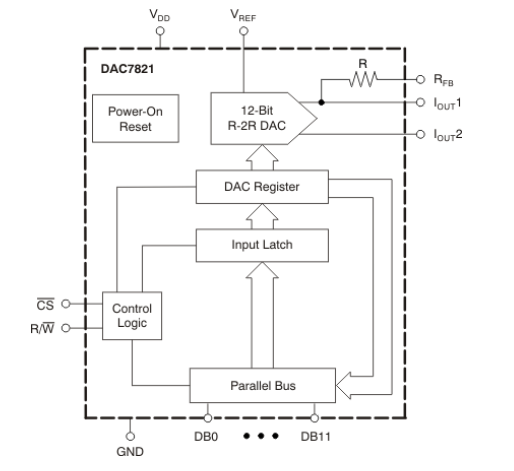
\includegraphics[width=\linewidth]{DAC7812.png}
        \caption{from Texas Instruments Data sheet }
        \label{fig:dac7812}
    \end{subfigure}\hspace{0.04\linewidth}
    \begin{subfigure}{0.35\linewidth}
        \centering
        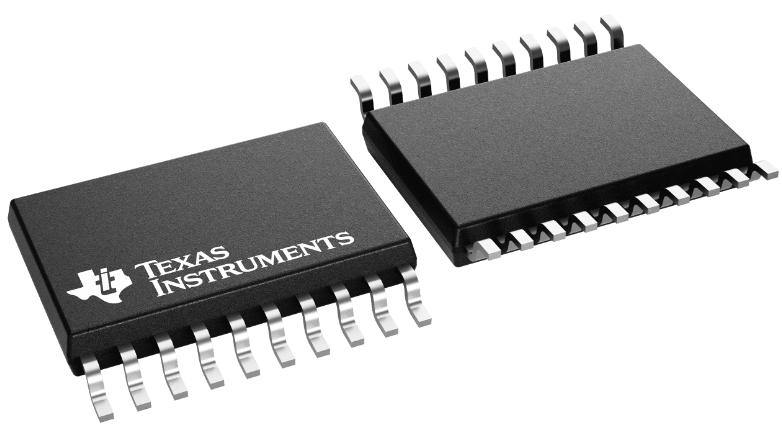
\includegraphics[width=\linewidth]{SMD.png}
        \caption{SMD}
        \label{fig:smd}
    \end{subfigure}
    \caption{DAC7812}
    \label{fig:combined}
\end{figure}

The DAC7821, a 12-bit DAC IC, employs an R-2R ladder network in conjunction with internal registers. Digital input codes are written to the Input Register, latched for stability, and processed through the ladder for analog conversion. Control bits in the Control Register manage operational modes, enabling precise analog output voltage control.
%%%%%%%%%%%%%%%%%%%%%%%%%%%%%%%%%%%%%%%%%%
\subsection{Key Features}

\begin{itemize}
    \item Resolution: 12 bits, Binary-Weighted Resistors.
    \item Fast Settling Time, Low Power Consumption.
    \item Wide Voltage Range.
\end{itemize}
%%%%%%%%%%%%%%%%%%%%%%%%%%%%%%%%%%%%%%%%%%
\subsection{Applications}

The DAC7821 finds applications in various fields, including industrial automation, audio systems, and instrumentation.


\end{document}
